\documentclass{article}
\usepackage{graphicx, amsmath, titlesec, titletoc, lmodern, algpseudocodex, ulem}
\usepackage[T1]{fontenc}
\usepackage{hyperref}
\hypersetup{
    colorlinks,
    citecolor=black,
    filecolor=black,
    linkcolor=black,
    urlcolor=black
}
\graphicspath{{figures/}}

\title{441 Final Notes}
\author{}
\date{}

% Remove section number from TOC
\titlecontents{section}[0pt]{\addvspace{1ex}\bfseries}
{}{}{\titlerule*[.5pc]{.}\contentspage}

\titlecontents{subsection}[10pt]{\addvspace{1ex}\bfseries}
{}{}{\titlerule*[.5pc]{.}\contentspage}

\titlecontents{subsubsection}[20pt]{\addvspace{1ex}\bfseries}
{}{}{\titlerule*[.5pc]{.}\contentspage}

% Remove section number from pdf
\titleformat{\section}{\normalfont\Large\bfseries}{}{0em}{}
\titleformat{\subsection}{\normalfont\large\bfseries}{}{0em}{}
\titleformat{\subsubsection}{\normalfont\normalsize\bfseries}{}{0em}{}

\begin{document}
\maketitle
\tableofcontents
\newpage

%------Chapter 3------%
\section{Chapter 3: Transport Layer}
\subsection{TCP}
At the transport layer, packets are delivered as segments. When client-server are connected via TCP
connection, the communication is bi-directional (even though there's only one connection) \\
\textbf{TCP Data Segment:}
\begin{itemize}
    \item \textit{Piggy backing:} a technique used by the \textbf{server} when setting up a TCP
    connection
    \begin{itemize}
        \item Client opens a TCP connection (request) with a server
        \item Server responds with an ACK (successful connection) and ontop of that, can send
        some data back
    \end{itemize}
    \item \textit{Sequence numbers:} Byte stream number of first byte in segment's data
    \item \textit{Acknowledgements:} Sequence number of next byte expected from otherside (cumulative ACK,
    similar to GBN)
    \item e.g. Host A and Host B sending data
    \begin{enumerate}
        \item $A\rightarrow\text{Seq}=92,\text{ data}=8\text{ bytes}\rightarrow B$
        \item $B\rightarrow\text{ACK}=100\rightarrow A$
        \item $A\rightarrow\text{Seq}=100,\text{ data}=20\text{ bytes}\rightarrow B$
        \item $B\rightarrow\text{ACK}=120\rightarrow A$
    \end{enumerate}
    \item TCP does not handle out-of-order packets, up to the implementors (discarding, buffering, etc)
\end{itemize}
To set up TCP's timeout value, it should be longer than RTT (even though it varies)
\begin{itemize}
    \item If t/o is too short $\rightarrow$ premature t/o $\rightarrow$ unnecessary retransmissions
    \item If t/o is too long $\rightarrow$ slow reaction $\rightarrow$ result in segment loss
\end{itemize}
To estimate RTT, we use \textbf{Sample RTT:} 
\begin{itemize}
    \item measured time from segment transmission until ACK reception (ignore retransmissions)
    \item Will vary (changes from packet to packet)
    \item Gaussian distribution to set RTT, a moving average 
    \[\text{EstRTT}=(1-\alpha)\times\text{CurrEstRTT}+\alpha\times\text{SampleRTT}\]
    \item Typical $\alpha=0.125$
    \item SampleRTT deviation from EstimatedRTT: 
    \[\text{DevRTT}=(1-\beta)\times\text{ DevRTT}+\beta\times|\text{SampleRTT}-\text{EstRTT}|\]
    \item Typical $\beta=0.25$ \[\text{T/oInterval}=\text{EstRTT}+4\times\text{DevRTT}\]
    \item Where EstRTT is the mean, DevRTT is the STD
\end{itemize}
TCP RDT at the \textbf{sending side:}
\begin{enumerate}
    \item \textit{Data from application layer:}
    \begin{itemize}
        \item Create a segment  with sequence number (goes into window)
        \item Start timer if not running already (begins with oldest unACKed segment)
    \end{itemize}
    \item \textit{Timeout:}
    \begin{itemize}
        \item Retransmit segment that cause t/o (not entire window)
        \begin{itemize}
            \item Restart timer $\rightarrow\text{EstRTT}+4\times\text{DevRTT}$
        \end{itemize}
        \item Expiration interval: TimeoutInterval (computed using SampleRTT)
    \end{itemize}
    \item \textit{ACK received:}
    \begin{itemize}
        \item If ACK acknowledges previous unACKed segment
        \begin{itemize}
            \item Update what is known to be ACKed
            \item Start timer if there are still unACKed segments
        \end{itemize}
    \end{itemize}
\end{enumerate}
Connection management in TCP: opening and closing a connection (handshake between sender/receiver)
\begin{itemize}
    \item \textbf{Opening:} 3 messages
    \item \textbf{Closing:} 4 messages
\end{itemize}
\newpage

%------Chapter 4------%
\section{Chapter 4: Network Layer (Data Plane)}
In this section, we are concerned with the \textbf{data plane (forwarding)} portion of the network layer. \\
\textbf{Data plane}
\begin{itemize}
    \item Also known as \textbf{fowarding}: Function is to move packets from the router input link to the output link
    \item \textit{Analogy:} The process of getting through a single interchange (turn)
    \item All information to do forwarding is in the router (localized operations)
    \item Determines how a datagram is forwarded to the appropriate output link
\end{itemize}

%----Router----%
\subsection{Router}
As mentioned above, the data plane forwards packets (datagrams at this layer) to the router's input
port and out the router's output port. Functionalities of the input and output port are as follows:
\begin{itemize}
    \item \textbf{Input}
    \begin{itemize}
        \item Bit-level reception (physical layer )$\rightarrow$ Ethernet (link layer) $\rightarrow$ decentralized 
        switching (network layer)
        \item At \textbf{decentralized switching}, use header field values to look up output port
        using the \textbf{forwarding table} in the input ports memory
        \item 2 approaches to \textbf{forward} datagrams:
        \begin{itemize}
            \item \textbf{Destination-based forwarding:} Forward based on destination IP address (traditional)
            \begin{itemize}
                \item Internet tries to match IP using \textbf{longest prefix matching} 
            \end{itemize}
            \item \textbf{Generalized forwarding:} Forward based on any set of header field values (implemented in SDN)
        \end{itemize}
        \item If datagrams arrive faster than forwarding rate, queue into \textbf{switch fabric}
        \begin{itemize}
            \item Transfers datagrams from input buffer to appropriate output buffer
            \item Switching rate is the rate at which packets can be transferred from in to out
            \item 3 types: \textit{memory, bus, crossbar}
        \end{itemize}
    \end{itemize}
    \item \textbf{Output}
    \begin{itemize}
        \item \textbf{Buffering} implemented when datagrams arrive from the switch fabric faster than
        the transmission rate
        \item \textbf{Scheduling discipline} chooses among queued datagrams for transmission (FIFO by default)
        \item Datagrams could be \textbf{lost} due to network \textbf{congestion} (lack of buffers)
        \item \textbf{Priority scheduling:} who gets best performance (network neutrality)
        \begin{center}
            \textcolor{red}{Q: So, how much buffering do we need?} \\
            \textcolor{blue}{A: Minimum amount of buffer because it is costly and consumes a lot of energy}
        \end{center}
        \item A good \textbf{rule of thumb} with regards to buffering:
        \begin{itemize}
            \item Average buffer = "typical" $RTT$ (~250 ms) $\times$ link capacity $C$
            \item E.g. $C=10$ GBps, $RTT=250$ ms = 0.25 s, $w=$ max cwindow
            \[w=C\times RTT=10\times0.25=2.5 \text{ GBit buffer}\]
        \end{itemize}
    \end{itemize}
\end{itemize}
\newpage

%----IP----%
\subsection{Internet Protocol (IP)}
A key function of an IP datagram is \textbf{fragmentation} and \textbf{reassembly}. These functions
exist because datagrams are large in terms of overhead, so links (at the link layer) are able to
transmit these packets.
\begin{itemize}
    \item Links have a \textbf{Max Transfer Unit} (MTU), which is the maximum size of a link \textbf{frame} 
    \item This means that datagrams$>$MTU have to be divided, via \textbf{fragmentation}
    \begin{itemize}
        \item One datagram becomes several smaller datagrams
        \item Once it reaches the destination, datagram is then \textbf{reassembled}
    \end{itemize}
    \item IP headers are used to identify fragments that are in order
\end{itemize}

%--Subnets--%
\subsubsection{Subnets}
Are equivalent to link layer LANs (a group of networks).
\begin{itemize}
    \item Use routers to connect networks together
    \item IP address is split into 2 parts [subnet address|host address] (high order, low order respectively)
    \item Hosts that are connected together without a router forms a \textbf{subnet}
    \begin{itemize}
        \item They share the same \textit{subnet address}, also known as the prefix
        \item e.g. 223.1.1.1, 223.1.1.2, 223.1.1.3, etc.
        \item A separate subnet could look like: 223.1.2.1, 223.1.2.2, 223.1.2.3, etc.
        \item These subnets can be connected to the same router via different interfaces (of the router)
        \begin{itemize}
            \item Connected via wired (Ethernet) or wireless (Wifi)
        \end{itemize}
    \end{itemize}
    \item As mentioned above, each interface of a router could form a subnet
    \item $2^8-2$ subnet addresses could be assigned to hosts, while there are 2 reserves:
    \begin{itemize}
        \item \textbf{Zero address:} host portion all 0's
        \item \textbf{Broadcast address:} host portion all 1's
    \end{itemize}
\end{itemize}
A protocol called \textbf{CIDR (Classless Inter-Domain Routing)} exists:
\begin{itemize}
    \item Subnet portion can be of any length
    \item IPv4 introduced classless to be able to allocate IP addresses more efficiently due to an IP address
    shortage
    \item Format: a.b.c.d/x where
    \begin{itemize}
        \item x: number of bits in the subnet portion
        \item Subnet portion: \textcolor{blue}{blue}, host portion: black
        \item e.g. \textcolor{blue}{11001000 00010111 0001000}0 00000000 $\rightarrow$ 200.23.16.0/23
        \item 23 indicates that there are 9 bits that can be assigned as host
    \end{itemize}
\end{itemize}
The way an IP address can be obtained is through an ISP. ISPs have a range of addresses that can be
purchased
\begin{itemize}
    \item ISPs condense their block into smaller blocks to give to organizations
    \begin{itemize}
        \item ISP block: 11001000.00010111.00010000.00000000 (200.23.16.0/20)
        \item Organization 1 block: 11001000.00010111.0001\textbf{000}0.00000000
        \item Organization 2 block: 11001000.00010111.0001\textbf{001}0.00000000
        \item Organization 3 block: 11001000.00010111.0001\textbf{010}0.00000000
        \item ...
        \item Organization 8 block: 11001000 00010111 0001\textbf{111}0 00000000
    \end{itemize}
    \item In this scenario, each organization will have 9 bits remaining to give to hosts, so 
    $2^9$ IP addresses can be distributed in each condensed (organization) block
\end{itemize}
ISPs get their block of addresses from an organization called ICANN (Internet Corporation for Assigned
Name and Numbers)
\begin{itemize}
    \item World wide organization in charge of IP address management
    \item Allocate addresses
    \item Manage DNS 
    \item Assign domain names, resolve disputes between domain names
\end{itemize}
\newpage

%--DHCP--%
\subsubsection{DHCP}
Hosts obtain an IP address either manually (hardcoded by the system admin) or via \textbf{DHCP (Dynamic Host 
Configuration Protocol)}.
\begin{itemize}
    \item A "plug-and-play" protocol, so we don't need to intervene (only server-side)
    \item Purpose is to allow hosts to dynamically obtain IP addresses from network servers when they join
    \begin{itemize}
        \item Since addresses can expire, a host can renew its lease with current address
        \item Can lease out addresses (if connected or "on")
        \item Once a host disconnects, address goes back into a pool of available IP addresses
    \end{itemize}
    \item It is an \textbf{application layer} protocol that uses \textbf{UDP}
    \item In action:
    \begin{enumerate}
        \item DHCP server formulates DHCP ACK containing client's IP, first hop router IP (for client),
        IP and name of DNS server
        \item Encapsulation of DHCP server, forward to client
        \item Client now knows its own IP, IP of first hop router, IP and name of DNS server 
    \end{enumerate}
\end{itemize}
When we don't know the IP of a DHCP server, we use a special IP called the \textbf{broadcast address}
(mentioned earlier).
\begin{itemize}
    \item Example IP: 10101100.00100000.00000000.00000000 (172.16.0.0/11)
    \item Broadcast addr: 10101100.00111111.11111111.11111111 (172.31.255.255)
    \item How it works:
    \begin{enumerate}
        \item Client \textbf{broadcasts} a DHCP request
        \item All DHCP servers discover this request, all respond
        \item Client chooses DHCP server to get IP from then \textbf{broadcasts} request
        \item Chosen DHCP server assigns IP, responds with a DHCP ACK
    \end{enumerate}
\end{itemize}
\newpage

%--NAT--%
\subsubsection{NAT}
Since IPv4 addresses are scarce (shortage of them), the goal of \textbf{NAT (Network Address Translation)}
is to be able use \textbf{one} IP address for an entire subnet
\begin{itemize}
    \item That is, one NAT IP source address of all packets leaving a subnet (at router interface)
    \item Private IP address blocks:
    \begin{itemize}
        \item Reserved by IANA for private Internets (not routable on global Internet)
        \begin{enumerate}
            \item IP: 10.0.0.0/8 $\rightarrow$ 10.255.255.255 ($2^24$ usable IP)
            \item IP: 172.16.0.0/12 $\rightarrow$ 172.31.255.255 ($2^20$ usable IP)
            \item IP: 192.168.0.0/16 $\rightarrow$ 192.168.255.255 ($2^16$ usable IP)
        \end{enumerate}
    \end{itemize}
    \item \textbf{Advantages:}
    \begin{itemize}
        \item Do not need a block of addresses from an ISP (1 for all devices)
        \item Can change addresses of devices in LAN without notifying the outside world
        \item Can change ISP without changing addresses of devices in LAN (private)
        \item Devices in LAN not explicitly addressable (not routable, good security)
    \end{itemize}
    \item How it works:
    \begin{enumerate}
        \item Sender creates a packet with src IP, port and dest IP, port
        \item Goes through a router. In the router, it:
        \begin{itemize}
            \item Records the local (private) IP and port number
            \item Replaces it with a public IP and random port number, then forward to destination
        \end{itemize}
        \item Receiver responds back with src IP and dest IP (public IP that was used) 
        \item Goes through router, router changes dest address back to local (private) IP
    \end{enumerate}
\end{itemize}
\newpage

%--IPv64--%
\subsubsection{IPv4}
The Internet standard (for now).
\begin{itemize}
    \item \textit{IP:} 32-bit identifier for host and router interfaces
    \item \textit{Interface (port):} Connection between host/router and physical link
    \begin{itemize}
        \item Routers have multiple interfaces (router ports)
        \item Hosts have one or two (wired Ethernet, wireless Wifi)
        \item NIC (hardware component)
    \end{itemize}
    \item Multiple interfaces means multiple IP addresses
    \item Represented in dotted decimal notation
\end{itemize}

%--IPv6--%
\subsubsection{IPv6}
Slowly being implemented in the Internet, but not fully because people found ways to keep IPv4 alive
(using CIDR, NAT, etc).
\begin{itemize}
    \item Instead of 32-bit addresses (IPv4), it uses 128-bit addresses
    \item Changes in the header format helped speed up processing and forwarding of packets
    \begin{itemize}
        \item Fixed 40-byte header
        \item No fragmentation
        \item No checksum
    \end{itemize}
    \item Since IPv4 is deployed everywhere (and IPv6 isn't), it's hard to make the switch immediately
    \item But, it does coexist with IPv4 through a method called \textbf{tunneling} (VPN is tunneling)
    \begin{itemize}
        \item IPv6 datagram carried as a \textbf{payload} in an IPv4 datagram among IPv4 routers
        \item IPv4 datagram essentially encapsulates an IPv6 datagram
    \end{itemize}
    \item How it works:
    \begin{itemize}
        \item Say we have 2 hosts running the IPv6 protocol, but in between there are strictly IPv4 routers
        \item A \textbf{dual stack} router exists, where it is able to handle IPv6 and IPv4 datagrams
        \item Host is connected to the IPv6 interface, IPv4 interface of the \textbf{dual stack} is connected
        to however many IPv4 routers are in between (creates the \textbf{tunnel})
        \item On the other end of the IPv4 router interface connects to another \textbf{dual stack}, which
        then connects to the other IPv6 host
        \item Logically, the \textbf{tunnel} acts as a channel that connects the two dual stack routers
        \item Encapsulation/de-encapsulation of the IPv6 datagram occurs at the IPv4 interfaces of the dual stack
    \end{itemize}
\end{itemize}
\newpage

%----Generalized forwarding and SDN----%
\subsection{Generalized Forwarding and Software-Defined Networking}
Generally, routers only care about the destination address (Generalized forwarding) of packets,
but SDN routers look at a combination of things and decides how it forwards these packets. \\
\textbf{SDN (OpenFlow)}
\begin{itemize}
    \item \textbf{OpenFlow} is an API used by SDN controllers to communicate with routers and applications
    running on network controllers
    \item Flow is defined by headers
    \item Generalized forwarding within SDN: simple packet handling rules
    \begin{itemize}
        \item Pattern: match values in packet header fields
        \item Actions for matched packet: drop, forward, modify, or send to controller
        \item This cannot be done in traditional routers
        \item Examples of pattern packet must match:
        \begin{enumerate}
            \item Drop: $src=1.2.*.*$, $dest=3.4.5.*$
            \item Forward: $src=*.*.*.*$, $dest=3.4.*.*$
            \item Send to controller: $src=10.1.2.3$, $dest=*.*.*.*$
        \end{enumerate}
    \end{itemize}
\end{itemize}
\newpage

%------Chapter 5------%
\section{Chapter 5: Network Layer (Control Plane)}
In this section, we are concerned with the \textbf{control plane (routing)} portion of the network layer. \\
\textbf{Control Plane}
\begin{itemize}
    \item Also known as \textbf{routing:} To determine the route taken by packets from the source to destination
    \item \textit{Analogy:} Process of planning a trip from home to the airport
    \item Has network-wide logic
    \item Two approaches to this: 
    \begin{itemize}
        \item \textbf{Traditional routing algorithms:} Implemented in routers and the most dominant (per-router control)
        \begin{itemize}
            \item Individual routing algorithms in every router interact with each other (to compute forwarding tables)
        \end{itemize}
        \item \textbf{Software-Defined Networking:} Implemented in (remote) servers (logically centralized control)
        \begin{itemize}
            \item Distinct controller interacts with its local Control Agents (CA) in routers (to compute forwarding tables)
        \end{itemize}
    \end{itemize}
\end{itemize}

%----Routing Algorithms----%
\subsection{Routing Algorithms}
Goal is to determine a \textit{'good' path} from src to dest via routers
\begin{itemize}
    \item \textit{good:} least cost, least congested, fastest
    \item \textit{path:} sequence of packets travese via routers from src to dest
    \item Classification of routing algorithms:
    \begin{itemize}
        \item Information:
        \begin{itemize}
            \item \textbf{Global (LS)}: All routers have complete topology and link cost information
            \item \textbf{Decentralized (DV)}: Routers know physically connected neighbors; is an
            iterative process where they can exchange information
        \end{itemize}
        \item Static/Dynamic
        \begin{itemize}
            \item \textbf{Static}: Routes change slowly over time
            \item \textbf{Dynamic}: Periodic update in response to link cost changes
        \end{itemize}
    \end{itemize}
\end{itemize}

%--Link State--%
\subsubsection{Link State: Dijkstra Algorithm}
\begin{itemize}
    \item Nodes (routers) know the entire topology as well as link costs to every other node
    \item Algorithm computes least cost paths from source node to all other nodes
    \item It is an \textbf{iterative} process
    \item Notation:
    \begin{itemize}
        \item $c(x,y)$: link cost from node $x$ to $y$, $c=\inf$ if not direct neighbors
        \item $D(v)$: current value of cost of path from source to dest $v$
        \item $p(v)$: predecessor node along path from source to dest $v$
        \item $N'$: Set of nodes whose least cost path is definitively known (keeps track of least cost paths)
    \end{itemize}
    \item Algorithm takes $O(n^2)$ time
\end{itemize}

%--Distance Vector--%
\subsubsection{Distance Vector (DV): Bellman-Ford Equation}
\begin{itemize}
    \item Dynamic programming (constant update)
    \item Each node has its own (as well as a copy of its neighbors) \textbf{distance vector} (DV)
    \begin{itemize}
        \item Nodes exchange this information periodically
        \item When a node receives a \textbf{new DV estimate} from its neighbor, updates its own 
        DV via BF equation
        \item When enough iterations are done, $Dx(y)$ will eventually become $dx(y)$
    \end{itemize}
    \item At each node,
    \begin{itemize}
        \item \textbf{Wait} for change in local link cost/message from neighbor
        \item \textbf{Recompute} estimates
        \item If DV to any dest has changed, \textbf{notify} neighbors
    \end{itemize}
    \item Notation:
    \begin{itemize}
        \item $dx(y)$: cost of least-cost path from $x$ to $y$, where \[dx(y)=min\{c(x,v)+dv(y)\}\]
        \item $min$: minimum taken over all neighbors $v$ of $x$
        \item $c(x,v)$: cost to neighbor $v$\
        \item $dv(y)$: cost from neighbor $v$ to dest $y$
        \item $Dx(y)$ (capital D): estimate of least cost from $x$ to $y$
    \end{itemize}
\end{itemize}

\subsubsection{Conclusion between LS and DV}
Overall takeaway:
\begin{itemize}
    \item \textbf{Link State}
    \begin{itemize}
        \item \textit{Message complexity:} Each node broadcasts link info to every other node
        \item \textit{Speed of convergence:} Very fast, $O(n\log n)$
        \item \textit{Robustness:}
        \begin{itemize}
            \item Node can advertise incorrect link cost
            \item Each node computes its own table
            \item More robust compared to DV
        \end{itemize}
    \end{itemize}
    \item \textbf{Distance Vector}
    \begin{itemize}
        \item \textit{Message complexity:} Exchange between neighbors only over several iterations
        \item \textit{Speed of convergence:} Generally slower than LS
        \item \textit{Robustness:} 
        \begin{itemize}
            \item Nodes can advertise incorrect link cost
            \item Each node's table used by another, error propagates through network
        \end{itemize}
    \end{itemize}
\end{itemize}
\newpage

%----Intra-AS Routing----%
\subsection{Intra-AS Routing}
Aggregate routers into regions known as "Autonomous Systems" (network), specifically 
\textbf{Intra-AS} routing. Forwarding table configured by intra/inter-AS algorithm
\begin{itemize}
    \item Determine entries for destinations within AS (and external)
    \item Routing among hosts and routers in the same AS
    \item All routers in the AS must run the \textbf{same} intra-domain protocol
    \item Routers in \textbf{different} AS can run different intra-domain protocols
    \item \textbf{Gateway router:} at the "edge" of its own AS, links to routers in other AS's
\end{itemize}
A few protocols to note:
\begin{itemize}
    \item \textbf{RIP (Routing Information Protocol):} one of the oldest, uses DV routing
    \item \textbf{IGRP (Interior Gateway Routing Protocol:)} CISCO, not used that much
    \item \textbf{OSPF (Open Shortest Path First:)} Same as IS-IS protocol, widely used
\end{itemize}

%--OSPF--%
\subsubsection{Open Shortest Path First (OSPF)}
\begin{itemize}
    \item \textit{Open:} publicly available
    \item Uses LS algorithm
    \begin{itemize}
        \item Has all the same features as LS (topology of routers, dijkstra's algorithm to compute)
    \end{itemize}
    \item \textit{Flooding:} OSPF LS broadcasts to all other routers in AS over IP
\end{itemize}
\newpage

%----Inter-AS Routing----%
\subsection{Inter-AS Routing}
Aggregate routers into regions known as "Autonomous Systems" (network), specifically 
\textbf{Inter-AS} routing. Forwarding table configured by intra/inter-AS algorithm.
\begin{itemize}
    \item Determine only external destinations for entries
    \item Routing among AS's
    \item \textbf{Gateways} perform inter-domain routing (as well as intra-domain)
\end{itemize}
Main protocol used in inter-AS routing:
\begin{itemize}
    \item \textbf{BGP (Border Gateway Protocol):} "Glue that holds the Internet together"
\end{itemize}

%--BGP--%
\subsubsection{Border Gateway Protocol (BGP)}
Biggest protocol (BGP) that makes the Internet, along side IP
\begin{itemize}
    \item \textit{eBGP (external):} obtain subnet reachability information from neighboring AS's
    routers
    \item \textit{iBGP (internal):} propagate reachability information to all AS-internal routers
    \item Goal is to determine good routes to other networks based on \textbf{reachability information} 
    and \textbf{policy}
\end{itemize}
\begin{figure}[htbp]
    \centering
    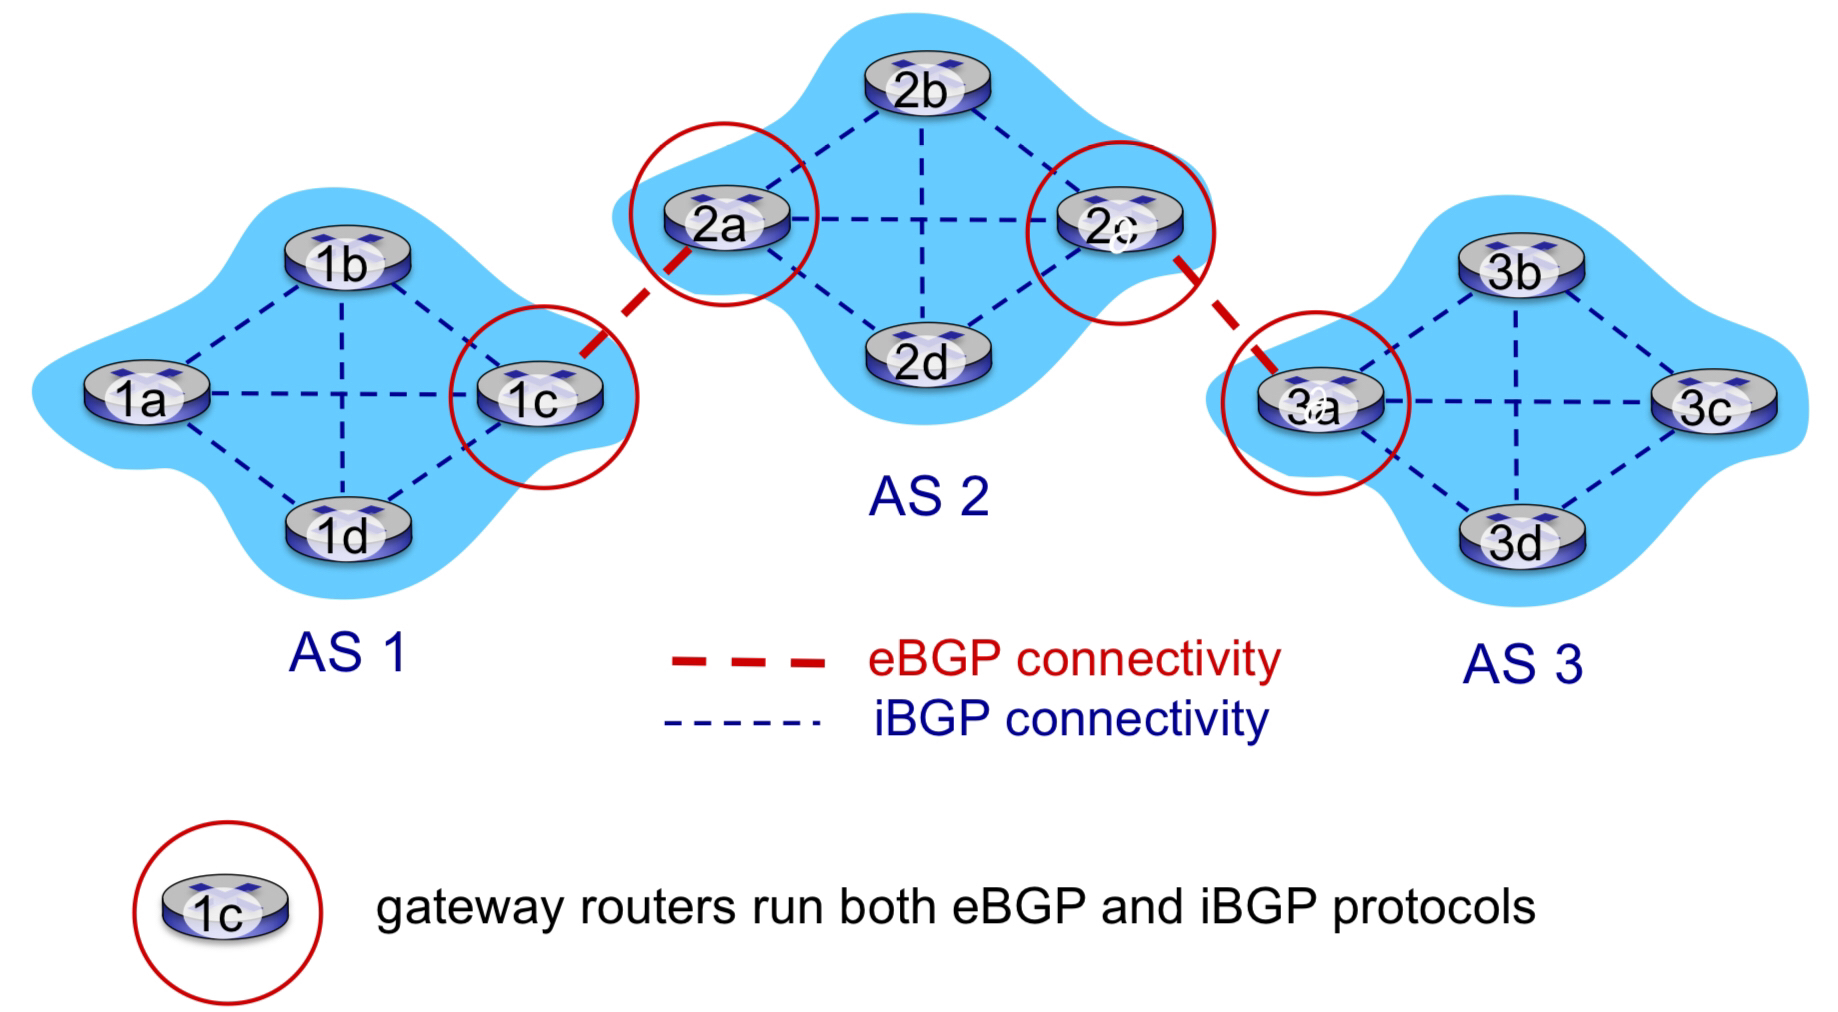
\includegraphics[width=1\textwidth]{interASconnection.png}
\end{figure}
\begin{itemize}
    \item \textit{BGP session:} Two BGP routers exchange BGP messages over a TCP connection
    \item It is a "path vector" protocol - it \textbf{advertises} paths to different destination
    network prefixes
    \item Important attributes with regards to advertised prefixes (prefix + attribute = "route")
    \begin{itemize}
        \item \textbf{AS-PATH:} list of AS's that has to be traversed to reach destination
        \item \textbf{NEXT-HOP:} Gateway router that advertised the route
    \end{itemize}
    \item For a node (from one AS) to reach another node (of a different AS), it has to go through 
    \textbf{gateway routers}
    \begin{itemize}
        \item Nodes learn this through advertised paths (mentioned above), which could present multiple
        paths
        \item A specific path is determined by a gateway router's policy
        \begin{itemize}
            \item If there are no specifications (by the gateway router), then the node chooses the
            shortest \textbf{AS-PATH}
        \end{itemize}
    \end{itemize}
    \item Hence, BGP \textbf{route selection} priority is as follows:
    \begin{enumerate}
        \item Local policy
        \item Shortest AS-PATH
        \item Closest NEXT-HOP router locally (not potato routing)
        \item Additional criteria
    \end{enumerate}
\end{itemize}
\textbf{Hot Potato Routing}
\begin{itemize}
    \item Chooses local gateway that has the least intra-domain cost
\end{itemize}
\newpage

%------Chapter 6------%
\section{Chapter 6: Link Layer}
\subsection{Overview}
The link layer is the second layer of the Internet Protocol stack. Some key words of 
this section include:

\begin{figure}[htbp]
    \centering
    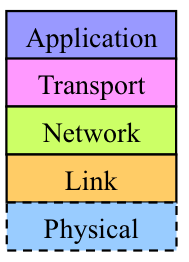
\includegraphics[width=0.2\textwidth]{IPstack.png}
    \caption{IP Stack}
\end{figure}

\begin{itemize}
    \item \textbf{Nodes} are what hosts and routers are referred to
    \item \textbf{Links} are communication channels that connect adjacent nodes along a 
    communcation path
    \begin{itemize}
        \item \textit{Wired} links (e.g. Ethernet)
        \item \textit{Wireless} links (e.g. Wifi)
    \end{itemize}
    \item \textbf{Frames} are what packets are called (encapuslates a network \textbf{datagram})
\end{itemize}
The link layer is responsible for transferring a datagram from one \textbf{node} to another
adjacent \textbf{node} via a \textbf{link}. Each link layer protocol (LLP) provides its own 
services (\textit{wireless wifi link, fiber optic link, copper link, etc}) but are \textbf{not guaranteed} to 
provide RDT/flow control, etc., over the link (upper layers are responsible). \\
As mentioned earlier, packets sent over to the link layer is called a link \textbf{frame}
\begin{itemize}
    \item It encapsulates a network \textbf{datagram} into a \textbf{frame}, adding its own 
    header fields
    \item Allows channel access if the medium is shared (e.g. shared link)
    \item Identifiers in \textbf{frame} headers are \textbf{MAC addresses} for source/destination
    (Completely different from IP!)
\end{itemize}
Reliable delivery between adjacent nodes were discussed in the transport layer of the stack. 
Though some links rarely use RDT (fiber optic), \textit{wireless} links have \textbf{very high error} 
rates. 
\begin{center}
    \textcolor{red}{Q: So, if RDT exists (TCP connection), would we still need end-end reliability?} \\
    \textcolor{blue}{A: Yes, because RDT at links are per hop (over nodes), so it does not guarantee data
    transfer over hosts.}
\end{center}
Some services the link layer provides include:
\begin{itemize}
    \item \textbf{Framing} and \textbf{Reliable delivery} (mentioned earlier)
    \item \textbf{Link access}
    \begin{itemize}
        \item No problems for \textbf{point-to-point} links
        \item Multiple Access Control (MAC) for shared links
    \end{itemize}

    \item \textbf{Flow control}
    \begin{itemize}
        \item Pacing between adjacent sending/receiving nodes (to prevent overflowing)
    \end{itemize}

    \item \textbf{Error Detection/Correction (EDC)}
    \begin{itemize}
        \item Errors caused by signal attenuation (loss of signal strength, e.g. noise)
        \item \textit{Receiver} detects presence of errors $\rightarrow$ signals sender for \textbf{retransmission}
        or \textbf{drop frame}
        \item \textbf{Correction:} Receiver identifies and correct bit errors \textbf{without} resorting
        to retransmission 
    \end{itemize}

    \item \textbf{Half/Full duplex}
    \begin{itemize}
        \item \textbf{Half:} Nodes \textit{cannot} simultaneously send/receive transmissions $\rightarrow$ one at a time
        \item \textbf{Full:} Nodes \textit{can} simultaneously send/receive transmissions
    \end{itemize}
\end{itemize}
The link layer is implemented in \textbf{every} node (host or router) via
\begin{itemize}
    \item \textbf{Adapter:} Network Interface Card (NIC)
    \item \textbf{Chip:} 5G, Bluetooth, etc.
\end{itemize}
The above are attached to a system bus, and it is a combination of hardware, software, and firmware. 
Adapaters communicate with each other, meaning one NIC communicates with another NIC (one sends
a frame while the other receives it).
\begin{itemize}
    \item \textbf{Sender:} Encapsulates datagram in frame then adds error checking bits, RDT,
    flow control, etc.
    \item \textbf{Receiver:} Looks for errors, RDT, flow control, etc. then extracts datagram, 
    passes it to the upper layers at receiving side
\end{itemize}
\newpage

%----EDC----%
\subsection{Error Detection and Correction (EDC)}
As mentioned earlier, \textbf{EDC} is one of the services provided by the link layer. Some variables
to note in this protocol:
\begin{itemize}
    \item \textbf{EDC:} Error detection and correction \textbf{bits} (AKA redundancy bits $\rightarrow$
    does not carry any information)
    \item \textbf{D:} The data protected by error checking, can also include header fields
\end{itemize}
While this service exists, it is \textbf{not 100\%} reliable. The protocol may miss some errors, but
rarely. To prevent this, use larger \textbf{EDC} fields for better detection and correction. When an
error is detected, frame could be dropped. \\
A couple of \textbf{EDC} protocols to note:

\begin{itemize}
    \item \textbf{Single Bit Parity Checking:}
    \begin{itemize}
        \item Detects single bit errors (cannot detect more than one)
        \item Uses the XOR ($\oplus$) operation at the receiver
        \item Two types:
        \begin{itemize}
            \item \textit{Even parity:} odd number of 1's, add 1 parity bit to make even 
            (e.g. 10110\textbf{1}$\leftarrow$parity bit)
            \item \textit{Odd parity:} even number of 1's, add 1 parity bit to make odd
        \end{itemize}
        \item \textbf{Advantages:}
        \begin{itemize}
            \item Simple to implemented
            \item Low overhead
            \item Fast calculation
        \end{itemize}
        \item \textbf{Disadvantages:}
        \begin{itemize}
            \item Can only detect one error (hence the name)
            \item Cannot correct error
        \end{itemize}
    \end{itemize}

    \item \textbf{2D Parity Checking:}
    \begin{itemize}
        \item Extended version of \textbf{single bit parity}, provides better detection AND does
        \textbf{correction} of the bit error
        \item Form of a 2D array (row parity and column parity), in the form of a 
        square matrix
        \item e.g. $D=101101101100$ (12 bits)
        \begin{center}
            \begin{tabular}{cccc|c}
                1 & 0 & 1 & 1 & 1 \\
                0 & 1 & 1 & 0 & 0 \\
                1 & 1 & 0 & 0 & 0 \\
                \hline
                0 & 0 & 0 & 1 & 1
            \end{tabular}
        \end{center}
        \item The above matrix shows 3 row parity bits on the right, 4 column parity bits at 
        the bottom, and 1 parity bit at the bottom right corner
        \item In total: $EDC=8$ additional bits along with $D=12$ bits.
        \item The way it detects an error bit is if a bit is flipped, both the row and column parities
        will be incorrect, \textbf{pinpointing} the incorrect bit.
        \item \textbf{Advantages:}
        \begin{itemize}
            \item Detects more errors than single bit parity
            \item Can locate the error bit
            \item Good at dealing with burst errors (confined within row/column)
        \end{itemize}
        \item \textbf{Disadvantages:}
        \begin{itemize}
            \item Does not detect ALL multi bit errors
            \item More overhead
        \end{itemize}
    \end{itemize}

    \item \textbf{Checksum (upper layer):}
    \begin{itemize}
        \item Adds 16 additional (redundancy) bits, making it stronger than parity
        \item \textbf{Sender side} caluclation:
        \begin{itemize}
            \item $D_1=01100110 10101010$, $D_2=11001100 00110011$
            \item Summation then one's complement (flip sum):
            \begin{center}
                \begin{tabular}{ccccccccccccccccc}
                    & 0 & 1 & 1 & 0 & 0 & 1 & 1 & 0 & 1 & 0 & 1 & 0 & 1 & 0 & 1 & 0 \\
                    & 1 & 1 & 0 & 0 & 1 & 1 & 0 & 0 & 0 & 0 & 1 & 1 & 0 & 0 & 1 & 1 \\
                    \hline
                    \textbf{1} & 0 & 0 & 1 & 1 & 0 & 0 & 1 & 0 & 1 & 1 & 0 & 1 & 1 & 1 & 0 & 1 \\
                    Carry out & & & & & & & & & & & & & & & & \textbf{1} \\
                    \hline
                    & 0 & 0 & 1 & 1 & 0 & 0 & 1 & 0 & 1 & 1 & 0 & 1 & 1 & 1 & 1 & 0 \\
                    \hline
                    1's comp. & 1 & 1 & 0 & 0 & 1 & 1 & 0 & 1 & 0 & 0 & 1 & 0 & 0 & 0 & 0 & 1
                \end{tabular}
            \end{center}
            \item Sender puts this in UDP checksum field
        \end{itemize}
        \item \textbf{Receiver side} calculation:
        \begin{itemize}
            \item Compute checksum of received \textbf{segment} (transport layer) 
            \item If computed checksum == checksum field value
            \begin{itemize}
                \item \textit{Yes:} No error (could potentially have)
                \item \textit{No:} Error detected
            \end{itemize}
        \end{itemize}
        \item \textbf{Advantages:}
        \begin{itemize}
            \item Simple
            \item Fast
        \end{itemize}
        \item \textbf{Disadvantages:}
        \begin{itemize}
            \item Not foolproof (even if no errors detected, errors could still exist)
            \item Cannot correct errors
        \end{itemize}
    \end{itemize}

    \item \textbf{Cyclic Redundancy Check (CRC):}
    \begin{itemize}
        \item Powerful error-detection protocol
        \item Uses modulo 2 arithmetic (add/subtract in XOR operation)
        \item \textbf{Sender side:}
        \begin{itemize}
            \item When calculating, we only care about the remainder (not the quotient)
            \item \textit{D:} Data bits (binary)
            \item \textit{G:} Generator (not an arbitrary number, shared between sender/receiver
            - hardcoded, given by $r+1$)
            \item \textit{R (or r):} CRC bits ($R=\text{remainder}[\frac{D\times2^r}{G}]$)
            \item Mathematical formula: $D\times2^r\oplus R$ (gets transmitted to \textbf{receiver})
        \end{itemize}
        \item \textbf{Receiver side:}
        \begin{itemize}
            \item Computes: 
            \[
            \frac{D\times2^r\oplus R}{G}=\frac{D\times2^r}{G}\oplus\frac{R}{G}=R\oplus R=0
            \]
        \end{itemize}
        \item Example:
        \begin{itemize}
            \item $D=101110$, $G=1001$ (because $G$ is 4 bits, $R=000$ is 3 bits)
            \item $D\times2^r\oplus R$, where $D\times2^r=101110[000]$
            \begin{center}
                \begin{tabular}{cccccccccc}
                    D: & 1 & 0 & 1 & 1 & \textcolor{red}1 & \textcolor{red}0 & \textcolor{green}0 & \textcolor{green}0 & \textcolor{blue}0 \\
                    G: & 1 & 0 & 0 & 1 \\
                    \hline
                    $\oplus$ & 0 & 0 & 1 & 0 & \textcolor{red}1 & \textcolor{red}0 \\
                    G: & & & 1 & 0 & 0 & 1 \\
                    \hline
                    $\oplus$ & & & 0 & 0 & 1 & 1 & \textcolor{green}0 & \textcolor{green}0 \\
                    G: & & & & & 1 & 0 & 0 & 1 \\
                    \hline
                    $\oplus$ & & & & & 0 & 1 & 0 & 1 & \textcolor{blue}0 \\
                    G: & & & & & & 1 & 0 & 0 & 1 \\
                    \hline
                    R: & & & & & & 0 & \textbf{0} & \textbf{1} & \textbf{1}
                \end{tabular}
            \end{center}
            \item Only take the first \textbf{3 bits} because that's all we need
            \item For transmission: 101110[011] where $D=101110$ and $R=011$
            \item At the receiver side, if we divide 101110[011] by \textit{G}, we should get 
            [000]
            \begin{itemize}
                \item If the remainder comes out to be non-zero, that means an error has been detected
            \end{itemize}
        \end{itemize}
        \item \textbf{Advantages:}
        \begin{itemize}
            \item Great at detecting errors (specifically burst)
            \item Quite efficient
            \item Standardized (Wifi, Ethernet)
        \end{itemize}
        \item \textbf{Disadvantages:}
        \begin{itemize}
            \item A lot more complex
            \item Cannot correct errors
        \end{itemize}
    \end{itemize}
\end{itemize}
To conclude: \textit{CRC, checksum, single bit parity check} \textbf{only detect errors} while \textit{2D parity
check} \textbf{detects errors and corrects them}.
\newpage

%----MAC----%
\subsection{MAC Protocols}
Multiple Access Control (MAC) links and protocols:
\begin{itemize}
    \item Point-to-point (link between Ethernet switch and host, PPP for dial up access)
    \item Broadcast (shared wire/medium)
\end{itemize}
Single-shared broadcast channel. If two or more nodes simultaneously transmit data, it results
in an interference (AKA a \textbf{collision}, which could result in packet - or frame - loss). To
prevent \textbf{collisions}, we have MAC protocols:
\begin{itemize}
    \item An algorithm that determines how nodes share a channel (when nodes can transmit)
    \item Communcation about channel sharing must \textbf{USE} the channel itself
\end{itemize}
Say we have a broadcast channel of rate $R$ bps. Ideally, we want:
\begin{itemize}
    \item Active nodes (N) to share equal bandwidth, given of rate $R/N$
    \item A single node to be able to fully utilize the channel, at rate $R$
    \item Fully decentralized (no special node to coordinate transmissions, no synchronization of
    clocks and slots)
    \item Simple to implement
\end{itemize}
3 MAC protocol techniques at the link layer:

%--Channel Partitioning--%
\subsubsection{Channel Partitioning}
\begin{itemize}
    \item Idea is to \textbf{prevent collisions}
    \item Divide channel into smaller pieces (hence the name)
    \item 2 procotols within this technique:
    
    \begin{itemize}
        \item \textbf{TDMA (Time Division Multiple Access)}
        \begin{itemize}
            \item Example: 6-station LAN
            \begin{itemize}
                \item Each station gets a fixed length slot, where length = packet transition time
                \item Unused slots go idle
                \item If only slots 1, 3, 4 have packets to send, we have wasted bandwidth at slots
                2, 5, 6 since slots are split equally
            \end{itemize}
            \item This technique is \textbf{only good} when there are nodes constantly using the channel
        \end{itemize}

        \item \textbf{FDMA (Frequency Division Multiple Access)}
        \begin{itemize}
            \item Instead of time slots, stations are divided into frequency bands
            \item Same idea as \textbf{TDMA}
            \begin{itemize}
                \item Station gets a fixed frequency band (slot)
                \item Unused bands go idle
            \end{itemize}
            \item Only good when nodes are in constant use of channels
        \end{itemize}
    \end{itemize}
\end{itemize}

%--Random Access--%
\subsubsection{Random Access}
\begin{itemize}
    \item Idea is to \textbf{detect and recover from collisions}
    \item Channel is \textbf{not} divided (purposely let collisions occur)
    \item Channels allows for full transmission rate for nodes
    \item A few protocols within this technique:
    
    \item \textbf{ALOHA}
    \begin{itemize}
        \item One of the oldest and simplest protocols, stemmed from the University of Hawaii
        by Norman Abramson in the 70s. Idea was to be able to route between islands
        \item \textbf{How it works:} 
        \begin{enumerate}
            \item User transmits whenever
            \item If two or more transmissions occur simultaneously, result in a \textbf{collision}
            \item Sender waits for an $RTT+\text{fixed delay}$ (No ACK = collision)
            \item Colliding stations retransmit packet, but stagger attempts randomly (probability) to reduce 
            repeated collisions
        \end{enumerate}
        \item Within this protocol, we have:
        \end{itemize}

        \item \textbf{\underline{Slotted ALOHA}}
        \begin{itemize}
            \item All frames have the same size
            \item Time is divided into equal sized slots - time to transmit \textbf{one frame}
            \item Nodes only transmit at the beginning of time slots
            \item Requires a clock synchronization (nodes are in sync, knows beginning and end of 
            time slots)
            \item Operation:
            \begin{itemize}
                \item When a node \textbf{receives} a frame, put it in a buffer and transmit
                at the \textbf{beginning of the next} time slot
                \item When a \textbf{collision occurs}, the node retransmits the frame in each
                subsequent time slot with a probability $p$ (system parameter) until success
                \item When there is \textbf{no collision}, the node can proceed to send the frame
                at the next time slot
                \item \textbf{Advantages:}
                \begin{itemize}
                    \item One active node can continuously transmit data at full rate of the channel
                    \item Decentralized (only slots in nodes need to be in sync)
                    \item Simple
                \end{itemize}
                \item \textbf{Disadvantages:}
                    \begin{itemize}
                        \item Collisions occur, wasted slots (idle slots if node has nothing to transmit)
                        \item Clock synchronization
                        \item The time it takes for a node to detect a collision may be less than the time
                        it takes for a frame to transmit
                    \end{itemize}
                \item \textbf{Efficiency:}
                    \begin{itemize}
                        \item $N$ nodes, $p$ probability, $R$ channel rate
                        \item Probability that a given node in a slot suceeds \[E=p(1-p)^{N-1}\]
                        \item Probability that \textit{any} node succeeds \[E=Np(1-p)^{N-1}\]
                        \item Probability for optimal efficiency (best case 37\%) \[E=(1-\frac{1}{N})^{N-1}=\frac{1}{e}=0.37\]
                        \item Throughput = $\frac{R}{e}$, Throughput for one node = $\frac{R}{e}\times\frac{1}{N}$
                    \end{itemize}
        \end{itemize}
    \end{itemize}

    \item \textbf{\underline{Pure ALOHA}}
    \begin{itemize}
        \item Simpler, no synchronization whatsoever
        \item When frame first arrives, immediately transmit
        \item Probability of collision increases - frame sent in current slot collides with frames sent
            in current - 1 and current + 1
        \item \textbf{Advantages:}
            \begin{itemize}
                \item Simple
                \item Decentralized
            \end{itemize}
        \item \textbf{Disadvantages:}
            \begin{itemize}
                \item Low throughput and high collisions
                \item Wasted bandwidth
                \item Delays
            \end{itemize}
        \item \textbf{Efficiency:}
        \begin{itemize}
            \item Probability that a given node succeeds \[E=p(1-p)^{2(N-1)}\]
            \item Probability for optimal efficiency (best case 18\%)\[E=\frac{1}{2e}=0.18\]
        \end{itemize}
        \item Main takeaway is that Slotted ALOHA is a lot more efficient than Pure ALOHA
    \end{itemize}

    \item \textbf{CSMA (Carrier Sense Multiple Access)}
    \begin{itemize}
        \item A way to improve \textbf{ALOHA} is to \textbf{listen} for packets in transmission
        \begin{itemize}
            \item If a channel is sensed to be \textbf{idle}, transmit entire frame
            \item If a channel is busy, defer transmission and wait for transmission of
            prior frame to finish
        \end{itemize}
        \item Although this is the idea, it does not entirely prevent collisions as \textbf{two}
        nodes could sense that a channel is idle (due to propagation delay and distance)
        \item Example:
        \begin{enumerate}
            \item Say nodes \textit{A, B, C, D} are on the same channel (link)
            \item Nodes $B$ and $D$ have data to transmit, sense that the channel is idle
            \item $B$ sends a frame miliseconds before $D$ - because the nodes are of the same
            channel, these transmissions are broadcasted to one another - but $D$ doesn't know that
            since the signal from $B$ hasn't been reached to $D$ yet
            \item Though it may result in a partial collision, signals that were collided may not
            be recoverable
        \end{enumerate}
        \item Two protocols under CSMA:
    \end{itemize}

    \item \textbf{\underline{CSMA/CD (Collision Detection)}}
    \begin{itemize}
        \item Can detect collisions fairly quickly (when detected, colliding transmissions are
        immediately aborted$\rightarrow$no channel waste)
        \item Implemented in \textbf{wired LANs} (Ethernet)
        \begin{itemize}
            \item Measures the signal strength and compares it with the transmission signal
            \item If the strengths are substantially different, collision detected
        \end{itemize}
        \item Harder to implement in \textbf{wirless LANs} (Wifi)
        \begin{itemize}
            \item Signals going in and out can be overwhelmed by other local transmissions
            \item Analogy: Turning on a flashlight in a well-lit room
        \end{itemize}
    \end{itemize}
    \item \textbf{Efficiency:}
    \begin{itemize}
        \item $t_{prop}=$ max propagation delay between 2 nodes (in a LAN)
        \item $t_{trans}=$ time it takes to transmit a frame (max-size)
        \item Efficiency equation: \[E=\frac{1}{1+5\frac{t_{prop}}{t_{trans}}}\]
        \item Efficiency reaches 100\% when:
        \begin{itemize}
            \item $t_{prop}$ goes to 0
            \item $t_{trans}$ goes to infinity
        \end{itemize}
        \item Performance is a lot better compared to ALOHA
    \end{itemize}
    \item \textbf{Advantages:}
    \begin{itemize}
        \item Simple
        \item Low overhead
        \item Decentralized
    \end{itemize}
    \item \textbf{Disadvantages:}
    \begin{itemize}
        \item Bad under heavy load
        \item Half-duplex (cannot do simultaneous transmission)
    \end{itemize}

    \item \textbf{\underline{CSMA/CA (Collision Avoidance)}}
    \begin{itemize}
        \item Idea is to allow nodes to \textit{reserve} a channel (avoid collisions of longer
        data frames)
        \item Implemented in \textbf{wireless LANs}
        \item \textbf{Sender and Receiver} 
        \begin{enumerate}
            \item First, \textbf{sender} transmits a small \textit{Request-To-Send} (RTS) 
            packet to \textbf{receiver} using CSMA
            \begin{itemize}
                \item RTS's may collide with each other (they're short frames)
            \end{itemize}
            \item \textbf{Receiver} broadcasts \textit{Clear-To-Send} (CTS) packet in response to
            the RTS
            \begin{itemize}
                \item Broadcast messages mean it's heard by all nodes in the LAN
            \end{itemize}
            \item \textbf{Sender} transmits data frame
            \item Other nodes defer any transmissions
        \end{enumerate}
        \item This is how a node \textit{reserves} a channel - via RTS-CTS message exchange, kind
        of similar to a handshake that terminates all other actions
    \end{itemize}
\end{itemize}

%--Taking Turns--%
\subsubsection{Taking turns}
\begin{itemize}
    \item Idea is to \textbf{implement the above 2}
    \item Two protocols:
    \item \textbf{\underline{Polling}}
    \begin{itemize}
        \item \textit{Master-Slave} relationship between nodes
        \begin{enumerate}
            \item \textit{Master} node gives permission (sends a request) to a \textit{slave} node
            \item \textit{Slave} node responds with either data or nothing
            \item \textit{Master} then moves onto the next node
        \end{enumerate}
        \item \textit{Slave} nodes have to wait for their turn - in chronological order
        \item Protocol is typically used for "dumb" devices (e.g. Bluetooth devices)
        \item \textbf{Advantages:}
        \begin{itemize}
            \item No collisions
            \item Fair access
        \end{itemize}
        \item \textbf{Disadvantages:}
        \begin{itemize}
            \item Polling overhead (consumes bandwidth even if node has no data to send)
            \item Latency (Turn based so nodes have to wait their turn)
            \item Single point of failure (If \textit{Master} fails, system fails)
        \end{itemize}
    \end{itemize}

    \item \textbf{\underline{Token Passing}}
    \begin{itemize}
        \item Idea was to get rid of the \textit{Master}
        \item It follows a ring topology, where nodes know their previous/next nodes
        \item A node starts with a \textit{control token} (packet), where they are free to transmit
        data
        \item The token is passed sequentially (in order)
        \item Used in industrial control
        \begin{itemize}
            \item If the current holder of the token has nothing to send, immediately pass the token
            to the next node
        \end{itemize}
        \item \textbf{Advantages:}
        \begin{itemize}
            \item No collisions
            \item Fair access
        \end{itemize}
        \item \textbf{Disadvantages:}
        \begin{itemize}
            \item Token overhead (consumes bandwidth even if node has no data to send)
            \item Latency (Turn based so nodes have to wait their turn)
            \item Single point of failure (If a node crashes with \textit{token})
        \end{itemize}
    \end{itemize}
\end{itemize}
To conclude: 
\begin{itemize}
    \item Channel Partitioning 
    \begin{itemize}
        \item TDMA: Time division
        \item FDMA: Frequency division
    \end{itemize}
    \item Random Access 
    \begin{itemize}
        \item ALOHA
        \item Slotted ALOHA
        \item CSMA
        \item CSMA/CD (wired, Ethernet)
        \item CSMA/CA (wireless, Wifi)
    \end{itemize}
    \item Taking Turns 
    \begin{itemize}
        \item Polling (Master-Slave)
        \item Token Passing
    \end{itemize}
\end{itemize}
\newpage

%----LANs----%
\subsection{Local Area Networks (LAN)}
A LAN is technically a subnet - a group of hosts, switches, etc. The difference between the two are:
\begin{itemize}
    \item \textbf{Subnets} are a part of the \textbf{network} layer
    \begin{itemize}
        \item Uses IP addresses (32-bit) to forward network datagrams
        \item Represented in dotted decimal notation
        \item Analogy: Social Insurance Number (does not change no matter where you are)
    \end{itemize}
    \item \textbf{LANs} are a part of the \textbf{link} layer
    \begin{itemize}
        \item Uses MAC addresses (48-bit) to forward link frames
        \item Represented in hexadecimal notation
        \item Analogy: Postal address (it changes geographically)
    \end{itemize}
\end{itemize}
Every host has a NIC adapter, and every NIC has a unique MAC address (arbitrary number). MAC addresses
are administered by the IEEE, and manufactureres obtain them by buying a portion of MAC address space.
MAC addresses do have some sort of life span (20 years), so they can be reused.
\begin{center}
    \textcolor{red}{Q: Why do we need a MAC address if we already have IP?} \\
    \textcolor{blue}{A: Not every network layer is an IP network layer}
\end{center}
This means that the \textbf{link} layer should work independently of the \textbf{network} layer.
The \textbf{link} layer cannot assume what kind of \textbf{network} will run above it. We also have
scenarios where a host doesn't have an IP address when it first joins a network (DHCP), so it'll need a way
to communicate with other nodes (via MAC)

%--Addressing--%
\subsubsection{Addressing}
As we know, a network datagram has IP addresses as its \textit{source} and \textit{destination}. When 
encapsulated by a link frame, since the link layer doesn't deal with any sort of IP, it has MAC 
addresses in the \textit{source} and \textit{destination} header fields. 
\begin{itemize}
    \item Example: At the network layer, host $A$ wants to send a datagram to host $B$
    \begin{enumerate}
        \item $A$ has $B$'s IP address, so in the datagram we have \textit{src: IP A} and 
        \textit{dest: IP B}
        \item Once we pass the datagram to the link layer, it gets encapsulated into a frame (header fields
        go from IP to MAC, so \textit{src: MAC A} and \textit{dest: MAC B})
        \item Only thing is, $A$ does not have the MAC address for $B$, so what do we do?
    \end{enumerate}
\end{itemize}
We use an addressing protocol:
\begin{itemize}
    \item \textbf{ARP (Address Resolution Protocol)}
    \begin{itemize}
        \item Every node runs ARP
        \item Has a feature called the ARP table (similar to a forwarding table at the network layer)
        \begin{itemize}
            \item Has parameters: <IP; MAC; TTL> (TTL: if mapping not used within given time, ~20min)
        \end{itemize}
        \item \textbf{Back to the scenario: Nodes communicating in the same LAN}
    \end{itemize}
    \begin{enumerate}
        \item $A$ wants to send $B$ a packet, has its IP but not its MAC (Not in $A$'s ARP table)
        \item $A$ will broadcast an \textit{ARP query} packet which contains $B$'s IP
        \begin{itemize}
            \item Destination MAC address will be FF-FF-FF-FF-FF-FF, where all nodes receives this query
        \end{itemize}
        \item Because the IP matches $B$'s IP, $B$ will respond to the sender, $A$, with its MAC address
        \begin{itemize}
            \item Frame will be sent to $A$'s MAC address (unicast)
        \end{itemize}
        \item $A$ will cache (save) $B$'s IP and MAC into the ARP table <IP B; MAC B; 20>
    \end{enumerate}
    \begin{itemize}
        \item Nice thing about ARP is that it is a "plug and play" protocol, so no intervention needed
        \item \textbf{Another scenario: Nodes communicating in a different LAN}
        \begin{itemize}
            \item Same thing, $A$ wants to communicate with $B$, but is separated by $R$ (router),
            so $A\rightarrow R \rightarrow B$
            \item Assume $A$ knows $B$'s IP
            \item Assume $A$ knows $R$'s IP (via DHCP, where it provides information of its local DNS
            and Gateway address)
            \item Assume $A$ knows $R$'s MAC (via ARP query with its Gateway address)
        \end{itemize}
        \begin{enumerate}
            \item $A$ creates a datagram with \textit{src: IP A} and \textit{dest: IP B}
            \item $A$ encapsulate datagram at link layer with \textit{src: MAC A} and \textit{dest: MAC R}
            but the payload still includes \textit{IP B} as destination
            \item Frame is received at $R$, de-encapsulates frame at network layer, sees 
            \textit{IP A} as source and \textit{IP B} as destination
            \item $R$ re-encapsulates datagram into frame but instead of \textit{src: MAC A}, the source
            is the MAC of the output interface that connected to $B$'s LAN (\textit{src: MAC R}, \textit{dest: MAC B})
            \begin{itemize}
                \item Output interface from $R$ has $B$'s mapping in its ARP table in this case, otherwise send an ARP query
                \item The frame still contains \textit{IP A} as its source in the payload
            \end{itemize}
            \item $B$ successfully receives frame
        \end{enumerate}
    \end{itemize}
\end{itemize}

%--Ethernet and Switches--%
\subsubsection{Ethernet and Switches}
The most dominant wired LAN (low cost NIC, first widely used LAN technology, fast transmission 
rates, uses CSMA/CD). \\
How Ethernet works:
\begin{itemize}
    \item An active switch exists in the center of connected hosts (via Ethernet)
    \item Each Ethernet link has its own protocol (nodes do not collide with each other, node per link)
    \item Hosts cannot see switches, think they are all directly connected to each other
    \item Ethernet frames (packets) of their own sort of structure:
    \begin{itemize}
        \item Same idea: except as mentioned earlier, NIC adapters communicate with one another, where
        it encapsulates an network datagram into an Ethernet frame
        \item Frame (at sender) includes the following:
        \begin{itemize}
            \item \textit{Preamble:} 7 bytes with pattern 10101010 followed by 1 byte with 10101011
            \begin{itemize}
                \item Used to synchronize the receiver with sender (not the actual time but ticks)
            \end{itemize}
            \item \textit{src and dest:} MAC addresses
            \item \textit{Type:} Indicates the upper layer protocol, usually IP
            \item \textit{Payload:} Data
            \item \textit{CRC:} Check if there are any errors (if yes, drop frame)
        \end{itemize}
    \end{itemize}
\end{itemize}
Although Ethernet is a direct link connection, it is said to be unreliable and connectionless
\begin{itemize}
    \item \textbf{Unreliable:} When a frame is received, no feedback is sent between NICs
    \begin{itemize}
        \item No ACK when frame is successfully received
        \item No NAK when fram is dropped
        \item This is where TCP (end-end reliability) comes into play, though errors are not very common
    \end{itemize}
    \item \textbf{Connectionless:} No handshaking done between NICs
\end{itemize}
Ethernet has its own MAC protocol:
\begin{itemize}
    \item \textbf{Unslotted CSMA/CD with binary backoff}
    \begin{itemize}
        \item Nodes are able to retransmit frame via binary (exponential) backoff
        \item Say we have 3 nodes: \textit{A, B, C}
        \begin{enumerate}
            \item Collision 1 occurs at $A$, so we want to retransmit frame
            \begin{itemize}
                \item $A$ is given a contention window of $k=[0,1]$
                \begin{itemize}
                    \item 0: $A$ will retransmit immediately
                    \item 1: $A$ will wait $k\times512$ bits, then retransmit
                \end{itemize}
                \item Hence, the probability of retransmission is $\frac{1}{2}$
            \end{itemize}
            \item Collision 2 occurs at $A$, want to retransmit (back to back)
            \begin{itemize}
                \item $A$'s contention window is doubled, $k=[0,1,2,3]$
                \begin{itemize}
                    \item 0: $A$ will retransmit immediately
                    \item Any other number: $A$ will wait $k\times512$ bits, then retransmit
                \end{itemize}
                \item Probability of retransmission is $\frac{1}{4}$
            \end{itemize}
            \item Collision 3 occurs at $A$, contention window doubled again, $k=[0,1,...,7]$, 
            probability of retransmission is $\frac{1}{8}$
            \item After the 10th retransmission attempt, contention window will no longer grow so
            $k=[0,1,...,1023]$ with probability $\frac{1}{1024}$
        \end{enumerate}
    \end{itemize}
\end{itemize}

%--Switches--%
Along with Ethernet, we have an device called a(n) (Ethernet) \textbf{switch}
\begin{itemize}
    \item Similar functionality as a router (it stores-forwards frames)
    \begin{itemize}
        \item Similar (if not, same) to the store-forward protocol, it selectively forwards frames
        given the MAC address
        \item Uses CSMA/CD to access a LAN segment (link)
    \end{itemize} 
    \item As mentioned earlier, it is practically invisible to nodes
    \item Also a plug-and-play device
    \item Is self-learning
    \item Hosts have a dedicated and direct connection to a \textbf{switch interface} (point-point)
    \item Since each host has its own dedicated link, there are no collisions amongst hosts connected 
    to a switch
    \item \textbf{Full duplex}, so hosts can simultaneously send/receive data without collisions
    \item \textbf{Switches} have a feature called a \textbf{switch table} (similar to a routing table)
    \begin{itemize}
        \item Parameters include: <MAC address of host; Interface to reach host; TTL>
        \item A \textbf{switch table} is initially empty, so it records entries every time a host
        sends a frame to another hosts
        \item Example: $A$ (connected via interface 2) wants to send frame to $B$ (connected via interface 5)
        \begin{enumerate}
            \item $A$ sends frame with destination $B$
            \item Table records entry <$A$; 2; TTL>
            \item Table does not have an entry for $B$, so it uses a technique called \textit{flooding}
            \begin{itemize}
                \item Switch forwards the frame to every node (except sender)
            \end{itemize}
            \item Table learns that $B$ is reachable via interface 5
            \begin{itemize}
                \item Now that there are entries for $A$ and $B$, \textit{selective forwarding} can be used
                (directly send frame without broadcasting)
            \end{itemize}
        \end{enumerate}
    \end{itemize}
    \item Same idea as interconnected switches - they become one big LAN
\end{itemize}

\end{document}
